\chapter{Future perspectives}\label{future}

This manuscript does not mark the end of the projects herein; the development of blik --- and of the ecosystem it lives in --- is ongoing, and much more is in the plans to further our understanding of \textit{D. radiodurans} and its key players, such as FtsZ and HU.

\localtableofcontents

\section{blik and napari}

The development of blik has already proven useful for daily use in our group and others.
However, there are several features that were part of blik's original plan, but which are not yet implemented, or only partially.
Other planned enhancements are not specific to blik, but more general napari features which will benefit blik and hopefully many other plugins and applications depending on napari.

\subsection{STA visualisation \textit{in situ}}
One of the main ones is the ability to visualise subtomogram averages \textit{in situ}, positioned and oriented based on the particle picks they originated from.
While some tools that can do this exist~\cite{ermelArtiaXElectronTomography2022}, they are either not fully interactive (particles cannot be selected, moved around, or isosurface levels changed), limited in performance, or both.
In order to develop this feature, some changes need to be done to napari to allow instance-based mesh and volume rendering.
Some of these changes are already partially implemented, and there are plans to continue on this development in the coming months.
Developing a generalized framework for such rendering in napari will also benefit several other fields where rendering of high numbers of instances at high performance is needed (molecular dynamics, highly-multiplexed labeling, astrophysics).

\subsection{3D interactivity}
3D interactivity in blik can still be significantly improved; some features planned for this purpose are:

\begin{enumerate}[noitemsep]
    \item particle picking on 3D slicing planes, without need to switch to 2D for accurate depth selection
    \item more ergonomic controls for orientation selection of picked particles
    \item improved two-way interaction between feature plots and 3D view (coloring, classifying, selecting particles)
\end{enumerate}

\subsection{Multicanvas}
Another crucial improvement for napari (and therefore blik) which is underway and has been on my --- and on other napari developers' --- to-do list is \href{https://github.com/napari/napari/issues/5348}{full support for multicanvas}.
Especially for segmentation and annotation, having access two linked views of 2D and 3D visualisations can make a big difference in the ergonomics of a tool.


\section{\textit{D. radiodurans}: FtsZ, HU, and more}

The ongoing efforts on HU and FtsZ encountered technical challenges that so far prevented us from reaching high resolution and unravel the structure and function of these proteins.
We already started to work around these challenges, and Harald Bernhard --- a postdoc in the MICA group --- has picked up the work on these projects and already started improving on it.
There are also new directions in which we'd like to extend our work on \textit{D. radiodurans}, using cryo-EM, cryo-ET and other imaging techniques; particularly, we're interested in understanding the effects of radiation damage on all these processes, and how \textit{D. radiodurans} protects itself from it.

\subsection{Chromatin and HU}

To increase our chances to identify and pick HU, a new dataset was collected with a phase plate, which allows to collect data closer to focus while improving the contrast of low spatial fequency information (\fullref{em_ctf}).
Preliminary results on this data showed more classes containing what could be HU in a similar conformation to what seen in \autoref{fig:hu_structure} (\autoref{fig:hu_blobs}).

\begin{figure}[ht]
    \centering
    \includegraphics[width=\textwidth]{other/hu_blobs.png}
    \titledcaption[HU+DNA: promising 2D classes]{Promising 2D classes from the phase plate dataset, potentially showcasing DNA in complex with HU.}
    \label{fig:hu_blobs}
\end{figure}

TODO: some hint on irina's ideas?

\subsection{FtsZ SPA}

Since Harald picked up this project, he has already managed to improve the results from the FtsZ+DDM dataset in a few ways.
With careful use of 2D and 3D classifications, it's possible to better isolate single filaments, which improves the initial model generation.
Balancing the different views by number of particles also improves the orientation distribution, reducing map artifacts at the cost of some global resolution.
Additionally, the use of a bigger box size in particle extraction has improved slightly the quality of the alignements and 2D class averages.
While the anisotropy issue remains, the new maps are much more interpretable, and match quite well those by \citet{fujitaStructuresFtsZSingle2023} from \textit{K. pneumoniae} FtsZ (\autoref{fig:ftsz_hari_map}).

\begin{figure}[ht]
    \centering
    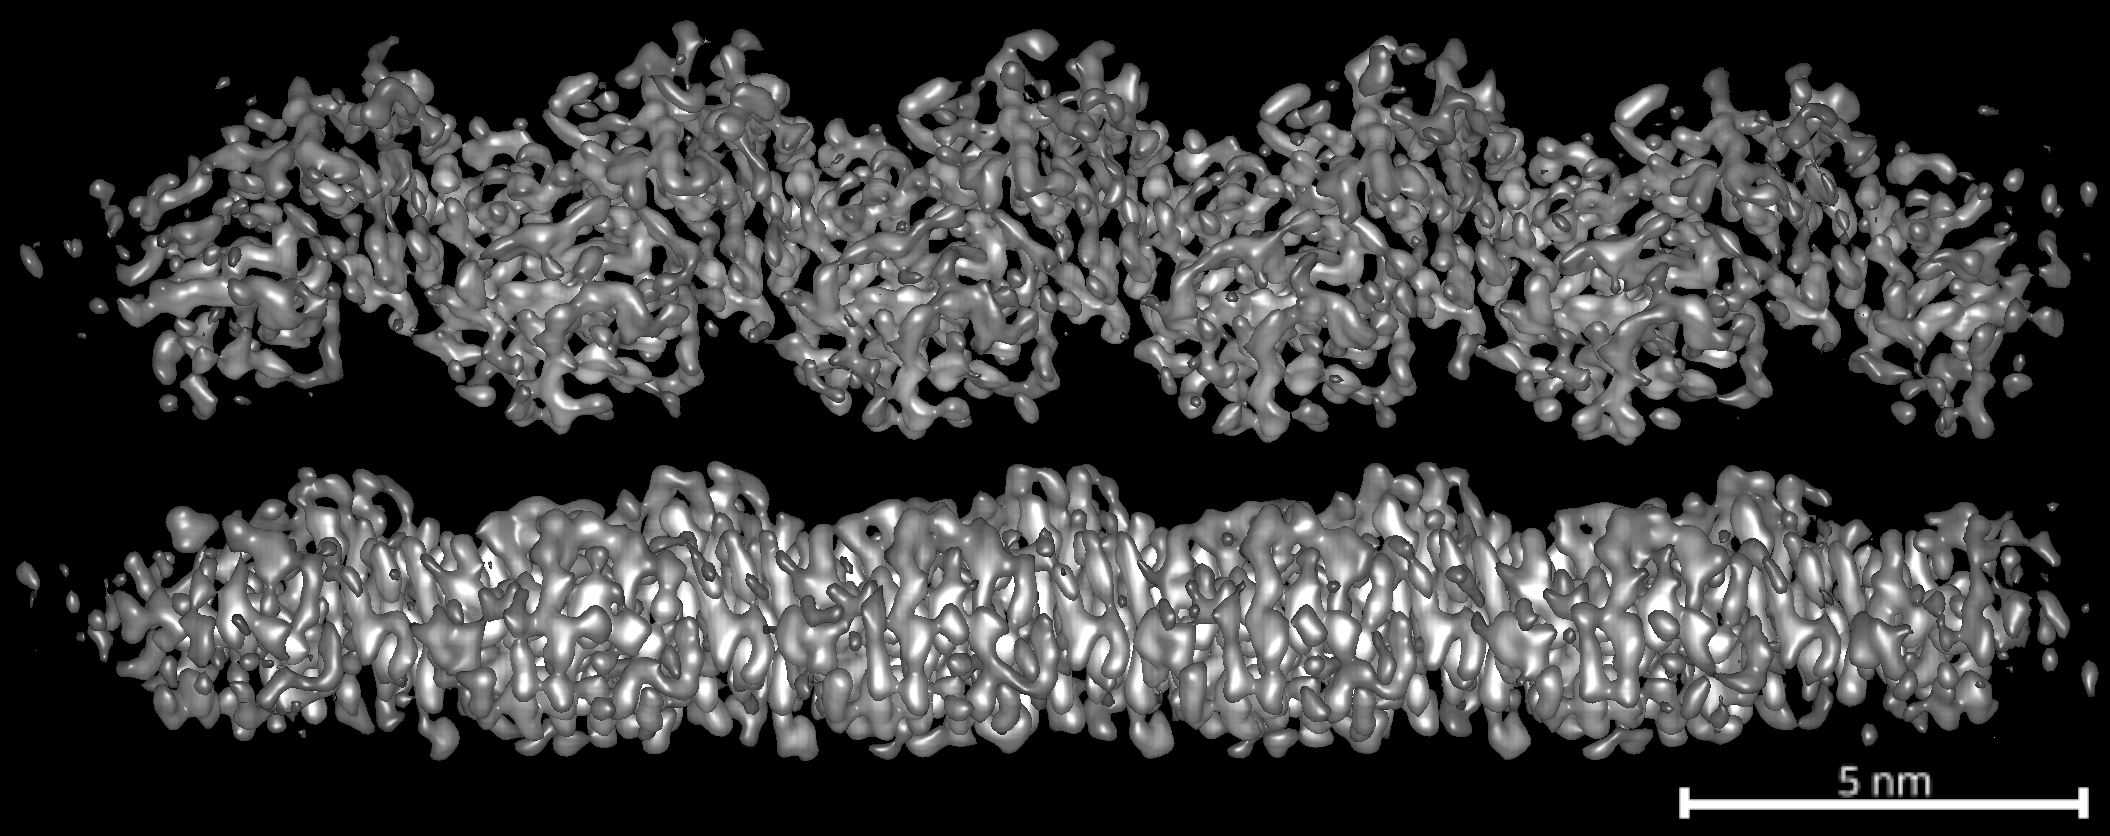
\includegraphics[width=\textwidth]{other/ftsz_map_good.png}
    \titledcaption[3D map of FtsZ with detergent]{Using the FtsZ+DDM dataset, and more careful 2D and 3D classifications to clean the dataset and better balance different views, Harald significantly improved on the FtsZ filament map. Preferential orientation is unfortunately still not fully solved, as evidenced by the streaking artifacts along one direction (bottom view), which are not present in the other (top view).}
    \label{fig:ftsz_hari_map}
\end{figure}

Depending on the outcome of the detergent dataset, we might need to go back to the tilted dataset.
We think that the process of assigning angles and restricting the search should be theoretically sound, so it may be worth spending more time tweaking parameters in Relion to find a working setup.
A recent study by ~\citet{aiyerOvercomingResolutionAttenuation2024} showed that negative effects of thickening the sample (due to tilting) should be negligible with proper preprocessing, so the achievable resolution should be unrestricted.

\subsection{FtsZ STA}

The cryo-ET dataset used in the septation paper (\fullref{drad}) was collected with the goal of capturing a wide field of view including a full \textit{D. radiodurans} cell.
For this reason, it contains a relatively low amount of FtsZ bundles (which are often not visible and/or not present in the lamellae), and has a relatively high pixel size (4.346 Å/px), which significantly limits our ability to reach high resolutions.

A new dataset has recently been collected by Irina with higher magnification and focused on the septa tips, which will hopefully provide a higher resolution view on the tips.

However, another problem with STA of FtsZ was the preferential orientation of the filaments, a consequence of how \textit{D. radiodurans} grows on the grid.
A way to tackle this problem is to force the bacteria into different orientations, for example by creating a dense paste of bacteria to freeze using the waffle method~\cite{kelleyWaffleMethodGeneral2022}.
Preliminary attempts to prepare such sample proved difficult to vitrify, but will be attempted again the future.

\subsection{Structural proteomics}

...


\section{Cryo-ET: state of the art and future directions}

what it's good for, what not

what changed in the field during this thesis (relion 5, warptools for linux, teamtomo, ai picking, 

scipion

cool stuff for future (MD + cryoet = awesome, generalized convention for per-particle tilt series and deformation fields etc)

\subsection{AI: Common pitfalls}

denoising, ai, important to look at things, to showcase

future with ML and AI in general?
